\documentclass{article}
\usepackage[utf8]{inputenc}
\usepackage{booktabs}
\usepackage{geometry}
\usepackage{pgfplots}
\pgfplotsset{compat=1.18}
\geometry{a4paper, margin=1in}

% Custom colors to match the reference chart style
\definecolor{strideblue}{RGB}{156,196,220}
\definecolor{lstmblue}{RGB}{95,160,205}
\definecolor{markovblue}{RGB}{63,133,186}
\definecolor{sgdpblue}{RGB}{21,61,122}

\begin{document}

% --- ORIGINAL COMPARISON TABLES ---
\begin{table}[htbp]
    \centering
    \caption{Hit Rate Comparison @ Cache Size 1000}
    \label{tab:hr_comparison}
    \begin{tabular}{lcccc}
        \toprule
        \textbf{Trace} & \textbf{No\_Pre} & \textbf{Stride} & \textbf{SGDP} & \textbf{GCN} \\
        \midrule
        mds\_0  & 69.99 & 83.37 & \textbf{89.18} & 86.86 \\
        proj\_0 & 11.02 & 73.97 & 78.50          & \textbf{84.04} \\
        src1\_2 & 26.85 & 66.34 & 83.27          & \textbf{86.14} \\
        hm\_1   & 92.77 & 96.80 & 97.66          & \textbf{98.42} \\
        prxy\_0 & 93.93 & 95.66 & 96.22          & \textbf{96.95} \\
        \bottomrule
    \end{tabular}

    \vspace{0.5cm}

    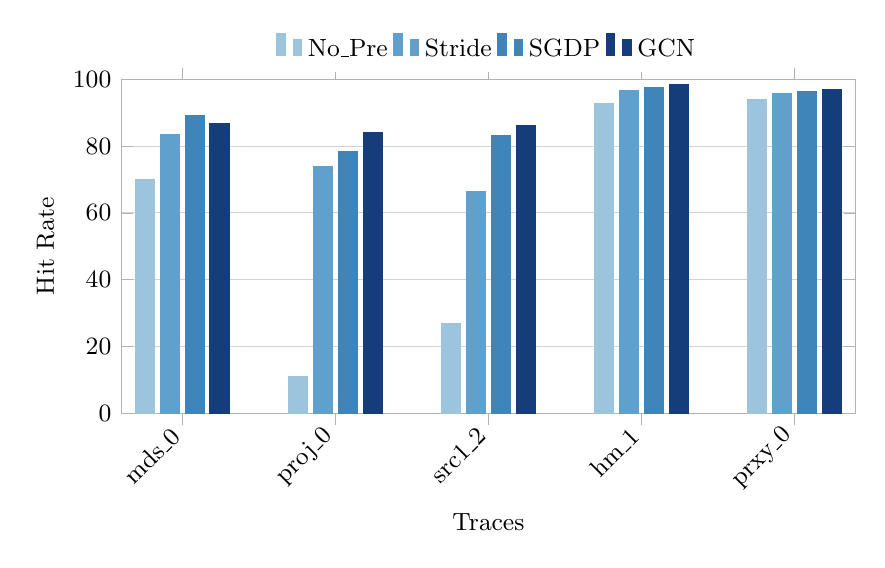
\begin{tikzpicture}
        \begin{axis}[
            ybar,
            bar width=7pt,
            width=0.90\textwidth,
            height=0.48\textwidth,
            ymin=0,
            ymax=100,
            ylabel={Hit Rate},
            xlabel={Traces},
            xtick={1,2,3,4,5},
            xticklabels={mds\_0, proj\_0, src1\_2, hm\_1, prxy\_0},
            x tick label style={rotate=45, anchor=east},
            tick label style={font=\small},
            label style={font=\small},
            legend style={
                at={(0.5,1.02)},
                anchor=south,
                legend columns=4,
                draw=none,
                font=\small
            },
            axis background/.style={},
            ymajorgrids=true,
            xmajorgrids=false,
            grid style={draw=gray!35},
            enlarge x limits=0.10,
            axis line style={draw=gray!60},
            tick style={draw=gray!60},
        ]
            \addplot[fill=strideblue, draw=strideblue] coordinates {(1,69.99) (2,11.02) (3,26.85) (4,92.77) (5,93.93)};
            \addplot[fill=lstmblue, draw=lstmblue] coordinates {(1,83.37) (2,73.97) (3,66.34) (4,96.80) (5,95.66)};
            \addplot[fill=markovblue, draw=markovblue] coordinates {(1,89.18) (2,78.50) (3,83.27) (4,97.66) (5,96.22)};
            \addplot[fill=sgdpblue, draw=sgdpblue] coordinates {(1,86.86) (2,84.04) (3,86.14) (4,98.42) (5,96.95)};
            \legend{No\_Pre, Stride, SGDP, GCN}
        \end{axis}
    \end{tikzpicture}
\end{table}

\begin{table}[htbp]
    \centering
    \caption{Prefetch Effectiveness Comparison @ Cache Size 1000}
    \label{tab:epr_comparison}
    \begin{tabular}{lcccc}
        \toprule
        \textbf{Trace} & \textbf{No\_Pre} & \textbf{Stride} & \textbf{SGDP} & \textbf{GCN} \\
        \midrule
        mds\_0  & 0.00 & 97.14 & 88.61          & \textbf{93.60} \\
        proj\_0 & 0.00 & 96.72 & \textbf{92.53} & 80.05 \\
        src1\_2 & 0.00 & 95.15 & \textbf{93.27} & 92.90 \\
        hm\_1   & 0.00 & 90.60 & 89.48          & \textbf{91.06} \\
        prxy\_0 & 0.00 & 92.31 & \textbf{82.00} & 53.32 \\
        \bottomrule
    \end{tabular}

    \vspace{0.5cm}

    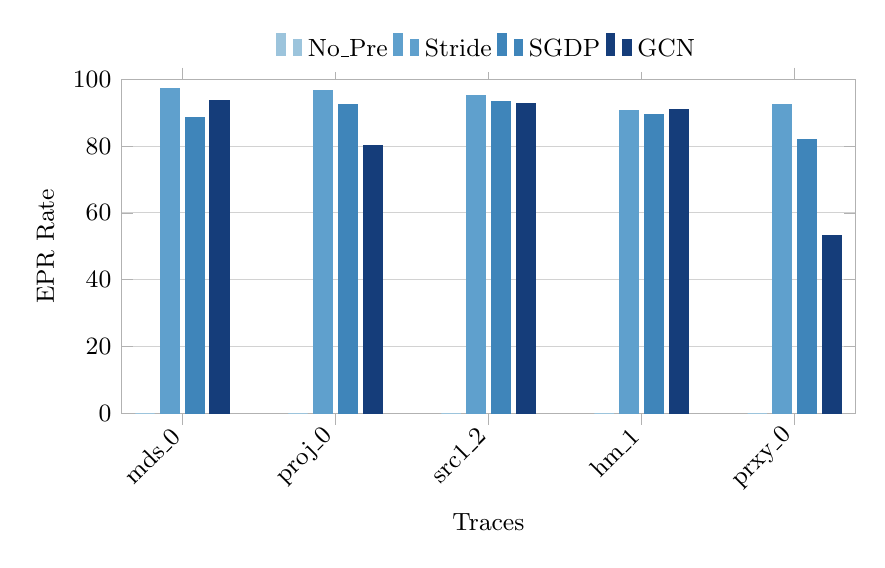
\begin{tikzpicture}
        \begin{axis}[
            ybar,
            bar width=7pt,
            width=0.90\textwidth,
            height=0.48\textwidth,
            ymin=0,
            ymax=100,
            ylabel={EPR Rate},
            xlabel={Traces},
            xtick={1,2,3,4,5},
            xticklabels={mds\_0, proj\_0, src1\_2, hm\_1, prxy\_0},
            x tick label style={rotate=45, anchor=east},
            tick label style={font=\small},
            label style={font=\small},
            legend style={
                at={(0.5,1.02)},
                anchor=south,
                legend columns=4,
                draw=none,
                font=\small
            },
            axis background/.style={},
            ymajorgrids=true,
            xmajorgrids=false,
            grid style={draw=gray!35},
            enlarge x limits=0.10,
            axis line style={draw=gray!60},
            tick style={draw=gray!60},
        ]
            \addplot[fill=strideblue, draw=strideblue] coordinates {(1,0.00) (2,0.00) (3,0.00) (4,0.00) (5,0.00)};
            \addplot[fill=lstmblue, draw=lstmblue] coordinates {(1,97.14) (2,96.72) (3,95.15) (4,90.60) (5,92.31)};
            \addplot[fill=markovblue, draw=markovblue] coordinates {(1,88.61) (2,92.53) (3,93.27) (4,89.48) (5,82.00)};
            \addplot[fill=sgdpblue, draw=sgdpblue] coordinates {(1,93.60) (2,80.05) (3,92.90) (4,91.06) (5,53.32)};
            \legend{No\_Pre, Stride, SGDP, GCN}
        \end{axis}
    \end{tikzpicture}
\end{table}

\begin{table}[htbp]
    \centering
    \caption{Inference Latency Comparison}
    \label{tab:latency_comparison}
    \begin{tabular}{lcc}
        \toprule
        \textbf{Trace} & \textbf{SGDP} & \textbf{GCN} \\
        \midrule
        mds\_0  & 1.194 & 0.040 \\
        proj\_0 & 0.694 & 0.045 \\
        src1\_2 & 0.717 & 0.041 \\
        hm\_1   & 0.699 & 0.043 \\
        prxy\_0 & 0.703 & 0.045 \\
        \bottomrule
    \end{tabular}

    \vspace{0.5cm}

    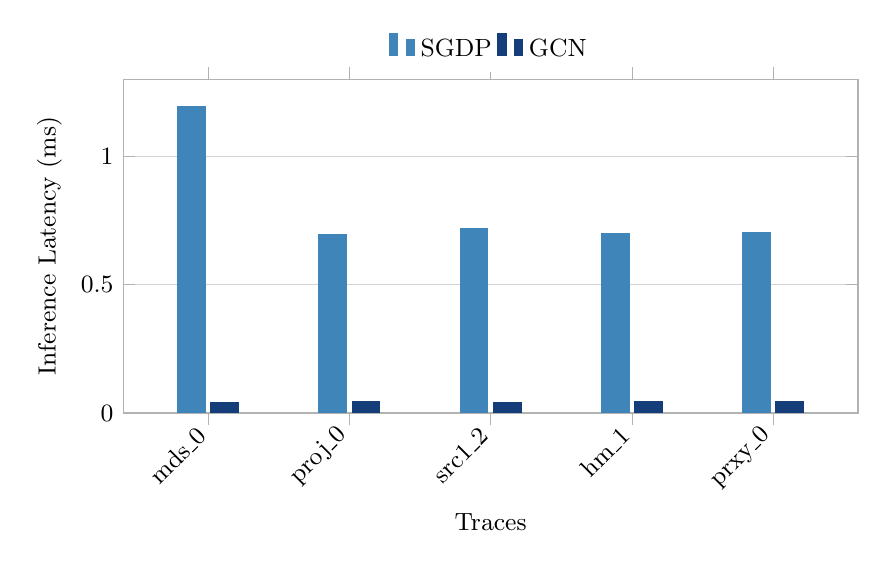
\begin{tikzpicture}
        \begin{axis}[
            ybar,
            bar width=10pt,
            width=0.90\textwidth,
            height=0.48\textwidth,
            ymin=0,
            ymax=1.3,
            ylabel={Inference Latency (ms)},
            xlabel={Traces},
            xtick={1,2,3,4,5},
            xticklabels={mds\_0, proj\_0, src1\_2, hm\_1, prxy\_0},
            x tick label style={rotate=45, anchor=east},
            tick label style={font=\small},
            label style={font=\small},
            legend style={
                at={(0.5,1.02)},
                anchor=south,
                legend columns=2,
                draw=none,
                font=\small
            },
            axis background/.style={},
            ymajorgrids=true,
            xmajorgrids=false,
            grid style={draw=gray!35},
            enlarge x limits=0.15,
            axis line style={draw=gray!60},
            tick style={draw=gray!60},
        ]
            \addplot[fill=markovblue, draw=markovblue] coordinates {
                (1,1.194) (2,0.694) (3,0.717) (4,0.699) (5,0.703)
            };
            \addplot[fill=sgdpblue, draw=sgdpblue] coordinates {
                (1,0.040) (2,0.045) (3,0.041) (4,0.043) (5,0.045)
            };
            \legend{SGDP, GCN}
        \end{axis}
    \end{tikzpicture}
\end{table}


\begin{table}[htbp]
    \centering
    \caption{Model Size Comparison}
    \label{tab:model_size_comparison}
    \begin{tabular}{lcc}
        \toprule
        \textbf{Metric} & \textbf{SGDP} & \textbf{GCN} \\
        \midrule
        Params & 261800 & \textbf{34768} \\
        \bottomrule
    \end{tabular}

    \vspace{0.5cm}

    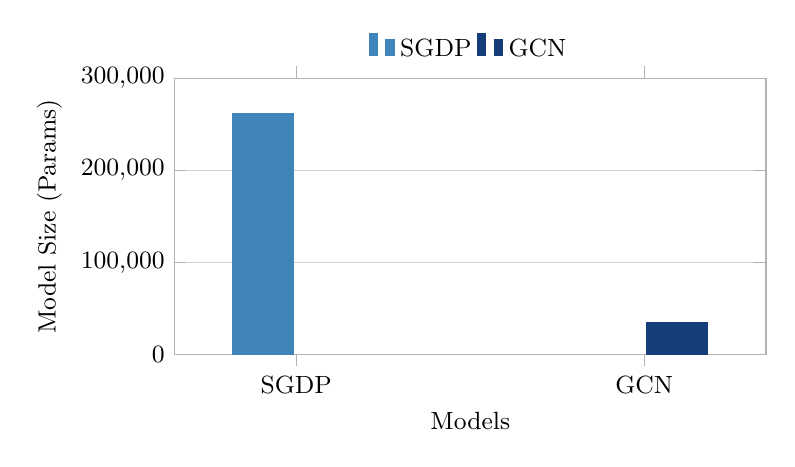
\begin{tikzpicture}
        \begin{axis}[
            ybar,
            bar width=22pt,
            width=0.75\textwidth,
            height=0.42\textwidth,
            ymin=0,
            ymax=300000,
            ylabel={Model Size (Params)},
            xlabel={Models},
            xtick={1,2},
            xticklabels={SGDP, GCN},
            tick label style={font=\small},
            label style={font=\small},
            legend style={
                at={(0.5,1.02)},
                anchor=south,
                legend columns=2,
                draw=none,
                font=\small
            },
            axis background/.style={},
            ymajorgrids=true,
            xmajorgrids=false,
            grid style={draw=gray!35},
            enlarge x limits=0.35,
            axis line style={draw=gray!60},
            tick style={draw=gray!60},
            scaled y ticks=false,
            yticklabel style={/pgf/number format/fixed, /pgf/number format/precision=0},
        ]
            \addplot[fill=markovblue, draw=markovblue] coordinates {(1,261800)};
            \addplot[fill=sgdpblue, draw=sgdpblue] coordinates {(2,34768)};
            \legend{SGDP, GCN}
        \end{axis}
    \end{tikzpicture}
\end{table}

\newpage
\section*{GNN Sensitivity Analysis Results}

% Table 3: Hit Rate
\begin{table}[htbp]
    \centering
    \caption{GNN Hit Rate (\%) for Different Layers and Hidden Sizes}
    \label{tab:gnn_hr}
    \begin{tabular}{lccc}
        \toprule
        \textbf{Hidden Size} & \textbf{1 Layer} & \textbf{2 Layers} & \textbf{3 Layers} \\
        \midrule
        16  & 98.410 & 98.400 & 98.340 \\
        32  & 98.450 & 98.420 & 98.300 \\
        64  & 98.390 & 98.420 & 98.390 \\
        128 & 98.390 & 98.370 & 98.430 \\
        256 & 98.440 & 98.440 & 98.340 \\
        \bottomrule
    \end{tabular}
\end{table}

% Table 4: Latency
\begin{table}[htbp]
    \centering
    \caption{GNN Inference Latency (ms) for Different Layers and Hidden Sizes}
    \label{tab:gnn_latency}
    \begin{tabular}{lccc}
        \toprule
        \textbf{Hidden Size} & \textbf{1 Layer} & \textbf{2 Layers} & \textbf{3 Layers} \\
        \midrule
        16  & 0.043 & 0.045 & 0.046 \\
        32  & 0.044 & 0.047 & 0.048 \\
        64  & 0.049 & 0.053 & 0.056 \\
        128 & 0.057 & 0.064 & 0.069 \\
        256 & 0.069 & 0.082 & 0.093 \\
        \bottomrule
    \end{tabular}
\end{table}

% Table 5: Prefetch Effectiveness
\begin{table}[htbp]
    \centering
    \caption{GNN Prefetch Effectiveness (EPR \%) for Different Layers and Hidden Sizes}
    \label{tab:gnn_pe}
    \begin{tabular}{lccc}
        \toprule
        \textbf{Hidden Size} & \textbf{1 Layer} & \textbf{2 Layers} & \textbf{3 Layers} \\
        \midrule
        16  & 91.850 & 92.090 & 91.580 \\
        32  & 91.220 & 92.160 & 94.370 \\
        64  & 93.410 & 94.070 & 93.040 \\
        128 & 93.320 & 94.140 & 93.230 \\
        256 & 93.360 & 93.420 & 93.110 \\
        \bottomrule
    \end{tabular}
\end{table}

\newpage
\section*{Averaged Performance by Layer}

\begin{figure}[htbp]
    \centering
    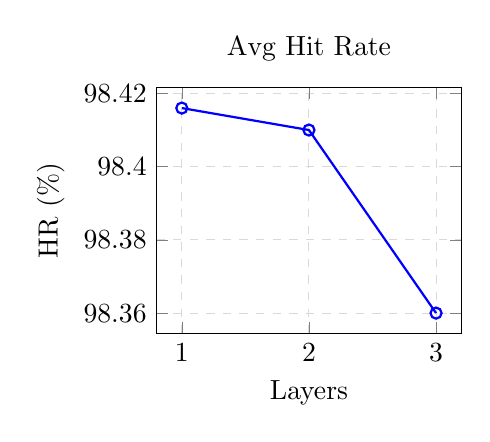
\begin{tikzpicture}
        \begin{axis}[
            width=0.45\textwidth,
            title={Avg Hit Rate},
            xlabel={Layers},
            ylabel={HR (\%)},
            xtick={1,2,3},
            grid=both,
            grid style={dashed, gray!30},
        ]
        \addplot[color=blue, mark=o, thick] coordinates {(1,98.416)(2,98.410)(3,98.360)};
        \end{axis}
    \end{tikzpicture}
    \hfill
    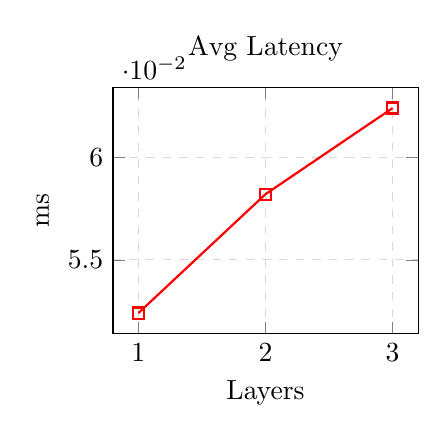
\begin{tikzpicture}
        \begin{axis}[
            width=0.45\textwidth,
            title={Avg Latency},
            xlabel={Layers},
            ylabel={ms},
            xtick={1,2,3},
            grid=both,
            grid style={dashed, gray!30},
        ]
        \addplot[color=red, mark=square, thick] coordinates {(1,0.0524)(2,0.0582)(3,0.0624)};
        \end{axis}
    \end{tikzpicture}
    
    \vspace{0.5cm}
    
    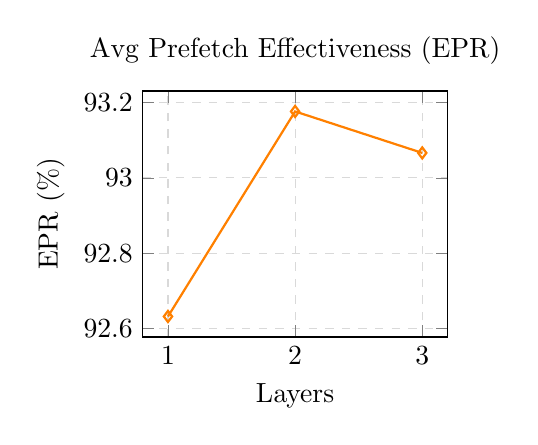
\begin{tikzpicture}
        \begin{axis}[
            width=0.45\textwidth,
            title={Avg Prefetch Effectiveness (EPR)},
            xlabel={Layers},
            ylabel={EPR (\%)},
            xtick={1,2,3},
            grid=both,
            grid style={dashed, gray!30},
        ]
        \addplot[color=orange, mark=diamond, thick] coordinates {(1,92.632)(2,93.176)(3,93.066)};
        \end{axis}
    \end{tikzpicture}
    \caption{Performance metrics averaged across all hidden sizes by model depth.}
\end{figure}

\section*{2-Layer GNN Scaling Analysis}

\begin{figure}[htbp]
    \centering
    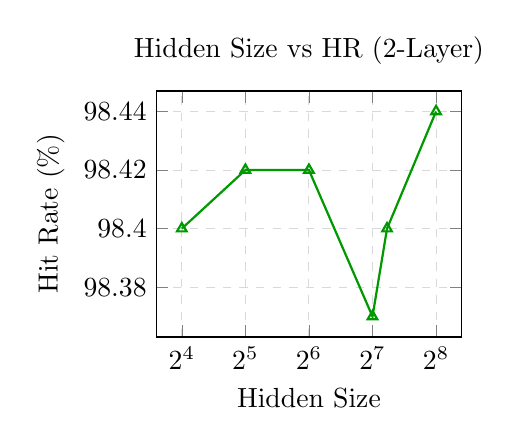
\begin{tikzpicture}
        \begin{axis}[
            width=0.45\textwidth,
            title={Hidden Size vs HR (2-Layer)},
            xlabel={Hidden Size},
            ylabel={Hit Rate (\%)},
            xtick={16, 32, 64, 128, 256},
            xmode=log, log basis x={2},
            grid=both,
            grid style={dashed, gray!30},
        ]
        \addplot[color=green!60!black, mark=triangle, thick] coordinates {
            (16, 98.40) (32, 98.42) (64, 98.42) (128, 98.37) (150, 98.4) (256, 98.44)
        };
        \end{axis}
    \end{tikzpicture}
    \hfill
    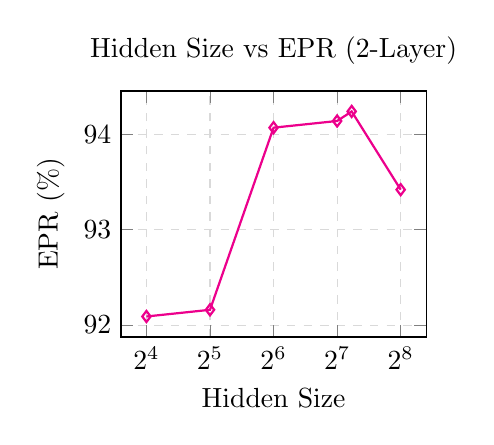
\begin{tikzpicture}
        \begin{axis}[
            width=0.45\textwidth,
            title={Hidden Size vs EPR (2-Layer)},
            xlabel={Hidden Size},
            ylabel={EPR (\%)},
            xtick={16, 32, 64, 128, 256},
            xmode=log, log basis x={2},
            grid=both,
            grid style={dashed, gray!30},
        ]
        \addplot[color=magenta, mark=diamond, thick] coordinates {
            (16, 92.09) (32, 92.16) (64, 94.07) (128, 94.14) (150, 94.24) (256, 93.42)
        };
        \end{axis}
    \end{tikzpicture}
    \caption{Scaling behavior of the 2-layer GNN configuration.}
\end{figure}

\end{document}